\section{Supplementary Screw Exploration Visualisations}
\label{sec:screw-exploration-figures}

The following figures support the exploratory screw-category experiments
described in Section~\ref{subsec:screw-exploration}.

% Figure 1
\begin{figure}[htbp]
\centering
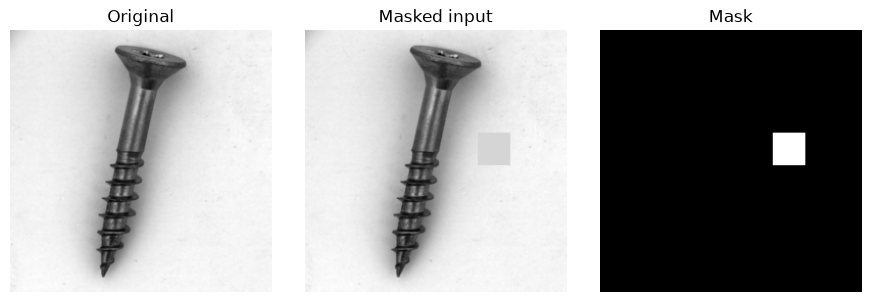
\includegraphics[width=0.7\textwidth]{figures/screw/figures/masking_example_background_miss.png}
\caption{Background-miss run. The masked $32\times32$ patch (right panel,
white square) sits almost entirely off the screw body, on plain background,
contributing little useful gradient signal about the object.}
\end{figure}

% Figure 2
\begin{figure}[htbp]
\centering
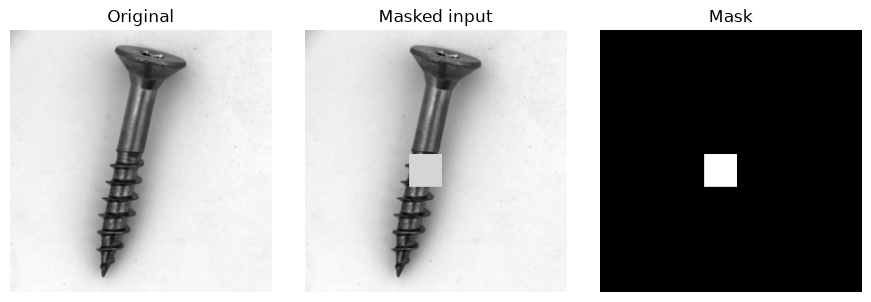
\includegraphics[width=0.7\textwidth]{figures/screw/figures/masking_example_object_hit.png}
\caption{Object-hit run. Same code, same patch size, a different unseeded
draw: the patch lands over the screw shaft, overlapping the object edge.
Same kernel behaviour, two different outcomes, illustrating the run-to-run
instability described in Section~\ref{subsec:screw-exploration}.}
\end{figure}

% Figure 3
\begin{figure}[htbp]
\centering
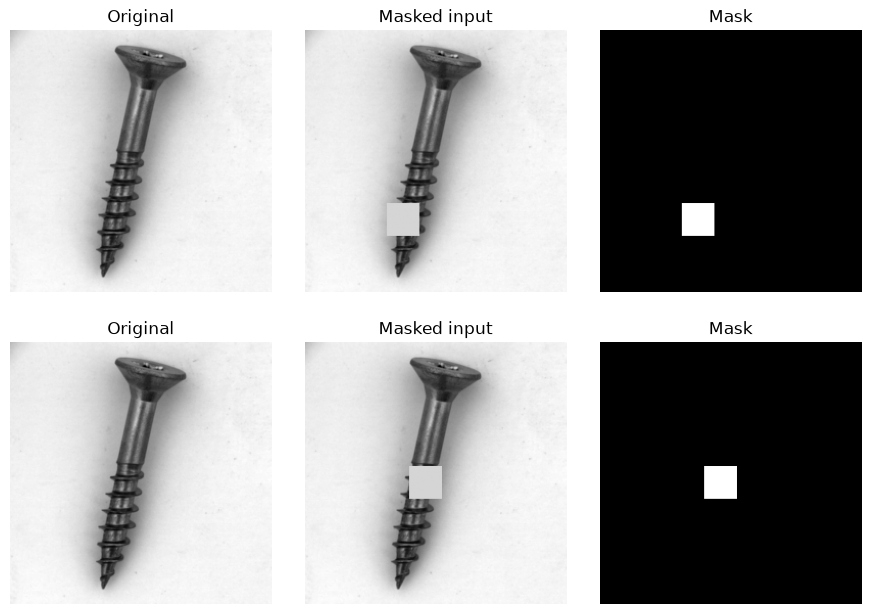
\includegraphics[width=0.7\textwidth]{figures/screw/fig_v3_masking_bug_vs_fix.png}
\caption{Top: Milestone S3's random masking lands mostly on background here.
Bottom: Milestone S4's object-centred masking places the patch on the screw.
Only the patch-placement rule differs.}
\label{fig:screw-masking-bug}
\end{figure}

% Figure 4
\begin{figure}[htbp]
\centering
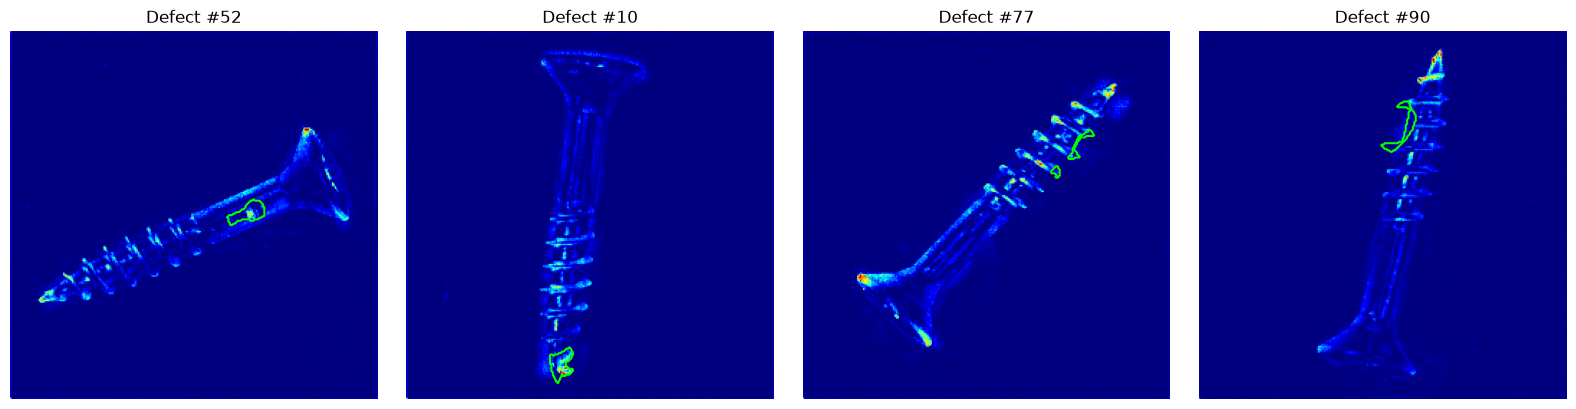
\includegraphics[width=0.85\textwidth]{figures/screw/fig_v2_localization_examples.png}
\caption{Green outline: true defect. Four defective screw test images with
Milestone S2's error heatmap. The mixed localisation illustrates the
AUROC/localisation disconnect discussed in
Section~\ref{sec:auroc_critique}.}
\label{fig:screw-localization}
\end{figure}

% Figure 5
\begin{figure}[htbp]
\centering
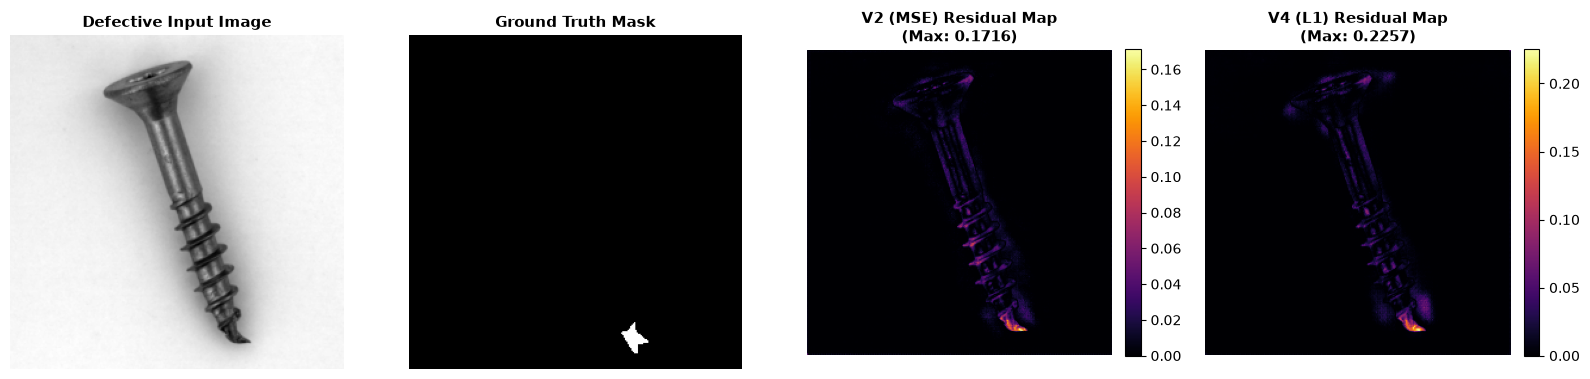
\includegraphics[width=0.85\textwidth]{figures/screw/fig_v2_v4_residual_snr.png}
\caption{The same defective screw test image scored by Milestone S2 (MSE)
and Milestone S5 (L1). The L1 residual is more concentrated on the actual
defect region. These pre-final checkpoints are illustrative rather than
confirmatory.}
\label{fig:screw-snr-map}
\end{figure}